\documentclass[11pt,a4paper]{article}

\usepackage{epsfig}
\usepackage{hyperref}


\begin{document}

\begin{titlepage}
\begin{center}

\textsc{\LARGE \bf{Software Requirements Specification}}
\textsc{\LARGE Computer Science Marks System}\\

\small Version: 0.3\\ \url{https://github.com/erosslee/COS301_MiniProject}

\vspace{0.5cm}
\textit{By group 10:}\\
Zenadia Groenewald (12265676)\\
Thulasizwe Mavuso (29236259)\\
Uteshlen Nadesan (28163304)\\
Z\"uhnja Riekert (12040593)\\
Estian Rosslee (12223426)\\
Moeletji Semenya (12349136)\\

\vspace{0.5cm}
\textit{For:} \\
Mr. Jan Kroeze (University of Pretoria)

\end{center}
\end{titlepage}
\newpage

\thispagestyle{empty}
\tableofcontents
\newpage

\setcounter{page}{1}
\pagestyle{plain}
\section{Introduction}
\textbf{(DONE by Zenadia - awaiting approval)}\\
The purpose of this requirements document is to identify and assess the specifications of the project, for the developers; as indicated by the client, the University of Pretoria’s Department of Computer Science. 
This document is to ensure that the requirements, specifications and scope of the project are understood and followed and to ensure that any and all parties involved understand the implications and understand what the final product should be capable of. This documents serves as an official contract and agreement between the developers and the client.

\section{Vision}
\textbf{(DONE by Z\"uhnja - needs to be checked)}\\
The main purpose of this project is that marks can easily be added directly to the university\textquoteright
s database through a user-friendly interface. No in between procedures.   Evaluators will be able to access the system with a mobile approach or via computer while they are assessing.  Students will be able to log into the system and view all of their marks. \\ \\
The client\textquoteright
s main aim with this project is to simplify and increase the efficiency of the marking system.
The project in question is meant to provide the Department of Computer Science with a sustainable and convenient system by which marks may be kept track of, changed and stored in a secure and efficient manner:
\begin{enumerate}
\item Store the marks of students registered for specific modules.
\item Keep track of the marks of registered students.
\item Track any and all changes made to marks at any point in time.
\item Track tutors assigned to courses and assessments.
\item Keep track of individual class/tutorial/practical/test averages as well as overall course averages.
\item Keep track of overall marks for individual students.
\item Update and display mark statistics in the form of graphs.
\item Store information regarding the privileges of lecturers and tutors.
\end{enumerate}This project scope serves as a basis for the project to expand for various similar applications with minimal changes necessary.

\section{Background}
\textbf{(DONE by Z\"uhnja, edited and amended by Zenadia - needs to be checked)}\\
This project is the result of the Department of Computer Science‘s need for their own improved marking system to potentially better the administration of students and their marks, and their decision to utilise the COS 301 course’s learning opportunity for the development of the required marking system; however it is also to prepare the developers for the larger undertaking of a similar task for external benefactors and stakeholders. These, among the aforementioned, have led to the development of this project:
\begin{enumerate}
	\item Potential business opportunities.
	\item The potential for work experience and skills development.
	\item The request of the clients to simplify/solve problems they are currently facing.
	\item Potential experience in how project development and business procedures work.
	\item The opportunity to learn how software development integrates with the business environment.
	\item Eliminating a common problems experienced by lecturers and students alike with regards to mark management and administration.
\end{enumerate}
Currently students view their marks for COS modules once they are posted on the CS website.  It is usually listed according to their student numbers; thus students are able to view each other's marks. 
During COS practical evaluations, markers evaluate each student's work and write their marks down on paper. That then has to be passed to someone who has the time to enter the marks into the University's system. In the process of this marking system the marks can easily get lost or be tampered with. \\
The aim of this project is to eliminate these threats. Marks won't have the opportunity to get lost, since they will be added to the system immediately. Students will be able to immediately access their marks once it is added to the system and they won't be able to view any marks that are not their own. 

\section{Stakeholders}
\textbf{(DONE by Moeletji - needs to be checked)}\\
The stakeholders invloved in this project are: 
\begin{itemize}
\item Mr. Jan Kroeze and the Department of Computer Science (client). 
\item Students and lecturers at the Department of Computer Science (end-users).
\item COS 301 students of 2014 (developers).
\item University of Pretoria -(organization). 
\end{itemize}

\section{Architectural requirements}
\textbf{(DONE by Thulasiswe - needs to be checked)}\\

\subsection{Access channel requirements}
The system's services are to be accessed by Android application clients and Browser clients through its web interface. These are the only two platforms that are to be supported by the system.

\subsection{Quality requirements}
\subsubsection{Performance}
	\begin{itemize}
		\item System must not take more than 1.5 seconds to return a searched for student.
		\item A request to view marks must be granted within 1.2 seconds.
		\item System must have auto complete mechanism for search services.
	\end{itemize}

	\subsubsection{Audit-ability}
	\begin{itemize}
		\item Every action on the system must be recorded on a log that can later be viewed and queried.
		\item Actions that are to be recorded
		\begin{itemize}
			\item The current user performing the action.
			\item New mark capturing.
			\item Deletion of marks.
			\item Edition of marks.
			\item Reason for editing the marks.
			\item The date/time on which an action was performed.
		\end{itemize}
	\end{itemize}

\subsubsection{Scalabity}
	\begin{itemize}
		\item The system must be able to be accessed by up to the current number of students registered for the course at any point.
		\item Additions and updates must be available to all the TA's when a mark sheet is unlocked.
	\end{itemize}	

	\subsubsection{Authorization}
	\begin{itemize}
		\item All actions are granted to a user based on the privileges they have.
	\end{itemize}

	\subsubsection{Authentication}
	\begin{itemize}
		\item The system must have an access control mechanism.
		\item Access control must be handled at log in/out points.
	\end{itemize}


\subsection{Integration requirements}
\subsubsection{MVC component communication}
\begin{itemize}
		\item The system will be built according Model-View-Controller(MVC) architectural design pattern.
			\begin{itemize}
			\item Model: The database with information about the system.
			\item View: The web interface and Android application.
			\item Controller: The SOAP interface.
			\end{itemize} 
		\item These components will need to communicate with each other and share information(using XML).
\end{itemize}
	\begin{itemize}
		\item Protocols that could be used:
			\begin{itemize}
			\item SOAP(for structred information exchange in a network)
			\item HTTPS(SOAP is going to rely on this protocol)   	
			\end{itemize}
		\item Quality Requirements
			\begin{itemize}
			\item Performance: Communication should happen in real-time.
			\item Reliability: Messages sent between components should be translated and structured correctly.
			\item Security: Messages should go from one component to another in the safest and simplest manner. 
			item Auditability: All communication between components should be recorded on an audit-log. 
			\end{itemize}	
	\end{itemize}

	
	\subsubsection{The Department of Computer Science website}
		\begin{itemize}
		\item Students and lectueres would only need to sign-in onto the CS website and they will automatically be signed-in onto the systems web-interface in order use the functions in 6.2.1.
		\item Protocols that could be used:
			\begin{itemize}
			\item LDAP(To help provide feature mentioned above)
			\end{itemize} 
		\item Quality Requirements	
			\begin{itemize}
			\item Security: Students or lecturers who cannot sign-in onto the CS website will be denied the services offered by the web-interface.
			\end{itemize}
	\end{itemize}
	
	\subsubsection{Fitchfork auto-marking system}
		\begin{itemize}
			\item The marking system would need to have an interface for communicating with Fitchfork in order to get marks.
			\item Protocols that could be used:
				\begin{itemize}
				\item TCP/IP(To specify how the two systems will communicate with each other)
				\item TSL/SSL(To provide security over the network when the two systems communicate)
				\end{itemize}	
			\item Quality Requirements
				\begin{itemize}
				\item Performance: The speed at which the two systems communicate should be realistic so when a practical auto-locks the marks are available for students to view.
				\item Security: Information communicated should not be intercepted or sniffed by user in the system.
				\item Reliability: The connection between systems must maintained when communicating.
				\item Auditability: Information on both the systems must correlate and be recorded. 	   
				\end{itemize}
		\end{itemize}
	

\subsection{Architectural constraints}
\textbf{(DONE by Thulasiswe - needs to be checked)}\\
\subsubsection{Technologies to be used}
	\begin{itemize}
		\item For the application platform
		\begin{itemize}
			\item Android SDK
			\item Java
		\end{itemize}
		\item For the web interface
		\begin{itemize}
			\item JavaScript
			\item HTML 4.0/HTML 5
		\end{itemize}
		\item Must be secure therefore must run over HTTPS
		\item Server side
		\begin{itemize}
			\item Django framework
			\item Python
		\end{itemize}
		\item Web service
		\begin{itemize}
			\item SOAP
		\end{itemize}
		\item MySQL for database
		\item LDAP for distributed directory information service
	\end{itemize}

\section{Functional requirements}
\subsection{Introduction}
The function of this project is to design an application interface that would enable a marker to upload the mark of a student, in a practical session, with his/her phone.
\subsection{Scope and Limitations/Exclusions}
\textbf {Use a high-level use case diagram with}\\
\subsubsection{Scope}
\textbf {Phone interface for the marker}

\begin{itemize}
\item Markers should only be able to view students who have registered for the specific practical period the marker is assigned to.
\item On specific markers with specific credentials should be able to log on to the application.
\item Markers can only log onto the application for their’ specified time slot and the application should run a check to provide this.
\item The marker should be able to look up the student being marked on his/her phone with either a student number or a first, last or both the first and last names of the student.
\item The interface should be simplistic and show the rubric and mark layout and have input boxes for the different mark fields.
\item For a change of a mark, the marker must provide a reason in the textbox that is saved for future reference.
\end{itemize}
\textbf{A web interface is also needed for lecturers and students}\\\\
\textbf{Lecturers:}

\begin{itemize}
\item Can only view records for courses they are in charge of.
\item Lock and unlock the database from being edited.
\item Need to be able to view records of marks as well as specific marks.
\item PDF documents for Lecturers should be generated detailing marks and 
descriptions.
\item Graphs of students’ marks should also be generated in the form of normal 
distributions, bar graphs and pie charts.
\item Counts of students should be available, as well as students registered standard 
deviations, averages and medians.
\end{itemize}
\textbf{Students:}
\begin{itemize}
\item Students should only be allowed to view their’ own marks and check their progress in the course thus far as well as overall progress with the course.
\item The student should not be able to edit marks.
\end{itemize}




\subsubsection{Limitations/Exclusions}
\begin{itemize}
\item No student should be able to view any mark besides their own.
\item The application should only be programmed for android smart phones.
\end{itemize}
\subsection{Required functionality}
\textbf{This application should be:}

\begin{itemize}
\item Accessible on android phones.
\item Scalable and viewable on devices.
\item Secure and information sent and received should be encrypted.
\item Auto log out after a specified time.
\end{itemize}

\textbf{The application:}
\begin{itemize}
\item Should have a database containing all students, lecturers and administrators as well as markers and a root user.
\item The root user should have access to all fields of the database. 
\item Should integrate with the automatic marker Fitchfork to receive specific student marks and be able to add these marks to a students’ mark database.
\item Should auto-complete names and student numbers being entered by markers. 
\item Generate CSV files for viewing and be able to accept CSV files of marks for input into the database of students marks.

\end{itemize}

\subsection{Use case prioritization}

\subsubsection{Critical: }
\begin{itemize}
\item The application needs to be functioning on the Android Platform and should be available on all Android phones for Android Version 2.0 upwards.
\item Marks must be able to be entered and uploaded to the server.
\item Have a web interface for viewing marks for students.
\item Have a web interface specific for lecturers.
\item Fitchfork integration.
\item Auto-lock the marks database from being edited 30 minutes to an hour after the practical session.
\end{itemize}

\subsubsection{Important: } 
\begin{itemize}
\item Good to exceptional performance speeds.
\item Encryption of communications.
\item Have a root user with unlimited access to the database and application. (The root user cannot edit audit-able documents)
\item Generated PDF documents with detailed reports.
\end{itemize}
\subsubsection{Nice-To-Have} 
\begin{itemize}
\item Auto-Complete.
\item Auto log off.
\item Student search via first name and/or surname.
\end{itemize}

\subsection{Use case/Services contracts}
For each use case/service specify
\\\\
\textbf{Pre-Conditions: }the conditions under which the service may be refused (usually there is an exception associated with each pre-condition).
\\\\
\textbf{Post-Conditions: }the conditions which must hold true after the service has been provided.
\\\\
\textbf{Request and Results Data Structures: }Use class diagrams to specify the data structure requirements for the request and result objects (i.e. the inputs and outputs).
\subsection{Process specifications}
For some of the use cases there may be requirements around the process which needs to be followed. If so, these requirements are typically specified via activity and/or sequence diagrams or
alternatively via state charts.
\subsection{Domain Objects}
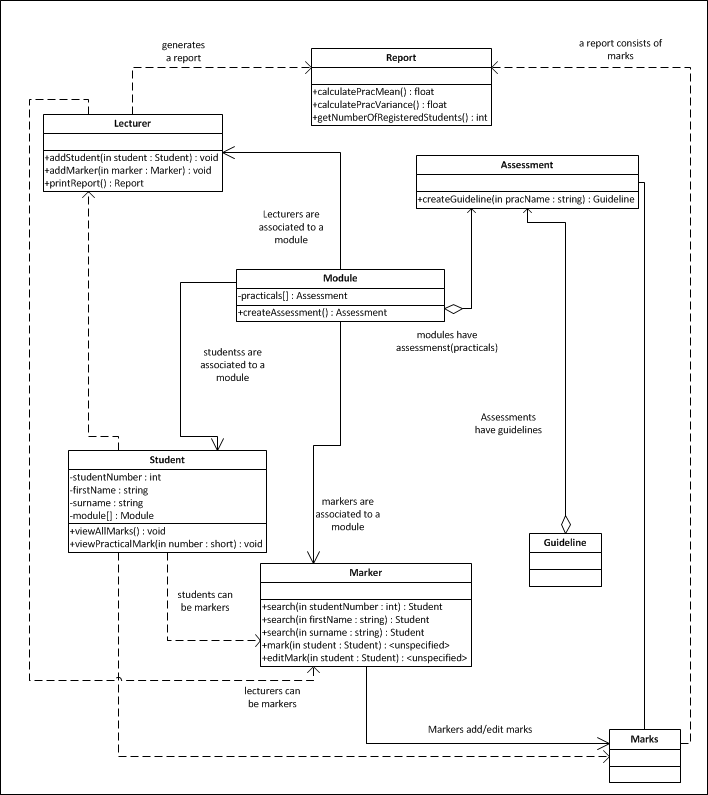
\includegraphics[width=1.0\linewidth]{Class_Diagram}
\\\\
Above is a class digram of the system with classes that contain attributes and methods in order to make the relatioships easier to comprehend. 
\section{Open Issues}
Discuss in this section
\begin{itemize}
	\item any aspects of the requirements which still need to be specified,
	\item around which clarification is still required, as well as
	\item any discovered inconsistencies in the requirements.
\end{itemize}
\section{Glossary}
The requirements is to be read, understood and validated by a range of people from very different backgrounds (the client, domain experts/business analysts, the developers, software architects, users, ... ). Use a glossary to explain any terms which some parties may not be familiar with.


\end{document}
